% Metódy inžinierskej práce

\documentclass[10pt,twocolumn,twoside,slovak,a4paper]{article}
%\documentclass[10pt,twoside,slovak,a4paper]{article}

\usepackage[slovak]{babel}
%\usepackage[T1]{fontenc}
\usepackage[IL2]{fontenc} % lepšia sadzba písmena Ľ než v T1
\usepackage[utf8]{inputenc}
\usepackage{graphicx}
\usepackage{url} % príkaz \url na formátovanie URL
\usepackage{hyperref} % odkazy v texte budú aktívne (pri niektorých triedach dokumentov spôsobuje posun textu)
\usepackage{graphicx}
\usepackage{caption}
\usepackage{subcaption}
\usepackage{cite}
\usepackage{amsmath}
%\usepackage{times}

\pagestyle{headings}

\title{Increasing Trade Efficiency through Recommendation Systems\thanks{Semestrálny projekt v predmete Metódy inžinierskej práce, ak. rok 2024/25, vedenie: Pavol Baťalík}} % meno a priezvisko vyučujúceho na cvičeniach

\author{Volodymyr Sorochynskyi\\[2pt]
	{\small Slovak University of Technology in Bratislava}\\
	{\small Faculty of Informatics and Information Technologies}\\
	{\small \texttt{xsorochynskyi@stuba.sk}}
	}

\date{\small September 19, 2024} % upravte


\begin{document}

\maketitle

\begin{abstract}
Recommendation systems are essential tools in modern business, enhancing customer interactions through personalized product and service offerings. Leveraging artificial intelligence algorithms and big data analytics, these systems allow trading platforms to deliver tailored recommendations based on user behavior, preferences, and similar customer data. This article explores how recommendation systems can improve store performance by personalizing the shopping experience and increasing user engagement. The focus is on analyzing the mechanisms used to provide personalized recommendations, as well as how different algorithms enhance conversion rates, average purchase value, customer retention, and overall satisfaction.

Additionally, the article examines the influence of recommendation systems on operational processes, such as inventory management and assortment optimization. The contributions of big data and artificial intelligence in refining recommendation accuracy and adapting to evolving consumer preferences are highlighted. Ethical considerations, including data privacy and the potential for recommendation bias, are also discussed. A key source for this research is Recommender Systems: The Textbook by Aggarwal (2016), which provides a comprehensive overview of the algorithms and their business impact.

In conclusion, recommendation systems have become integral to successful business strategies, allowing companies to increase sales, improve customer interaction, and optimize inventory management, while also necessitating careful attention to evolving privacy and ethical issues.
\end{abstract}

\begin{figure}[htbp]
    \centering
    
\includegraphics[width=0.3\textwidth]{logo.jpg}
    \caption{FIIT Logo}
    \label{fig:fiit_logo}
\end{figure}


\section{Introduction}

In today’s global economy, trade efficiency is a critical factor for success. Whether in local markets or international exchanges, the ability to streamline trade processes, reduce costs, and improve accuracy can significantly enhance profitability and competitiveness. Technological advancements have played a key role in driving improvements in trade efficiency, enabling businesses to operate more effectively in an increasingly complex environment.

One such technological advancement is the use of \textit{recommendation systems}. Originally designed to improve customer experiences in e-commerce, media, and entertainment industries, recommendation systems are now being explored for their potential to revolutionize trade processes. By leveraging vast amounts of data and sophisticated algorithms, these systems can provide personalized suggestions and insights that help businesses optimize their trade strategies, discover new opportunities, and improve decision-making.

This article explores how recommendation systems can be applied to enhance trade efficiency, examining their role in improving the speed, cost-effectiveness, and overall outcomes of trade operations.



\section{Understanding Trade Efficiency}

Trade efficiency refers to the effectiveness with which goods and services are exchanged in markets, both domestically and internationally. A highly efficient trade system enables quicker transactions, reduces costs, minimizes errors, and maximizes profits. Efficiency in trade is influenced by various factors, including:

\begin{itemize}
    \item \textbf{Cost:} Reducing transaction costs, tariffs, and shipping expenses contributes to greater efficiency.
    \item \textbf{Speed:} Faster processing times for orders, payments, and deliveries improve trade efficiency by minimizing delays.
    \item \textbf{Accuracy:} Correct and up-to-date information about products, pricing, and availability helps avoid costly mistakes and miscommunication.
    \item \textbf{Market Access:} The ability to easily connect with a broader range of buyers and sellers increases trade opportunities and boosts efficiency.
\end{itemize}

\noindent In the past, businesses have relied on traditional methods to enhance trade efficiency, such as improving supply chain management, optimizing inventory systems, and using more effective marketing strategies. While these methods have had a significant impact, the rapid growth of digital technologies has opened up new avenues for driving trade efficiency, especially through data-driven approaches.

In this context, recommendation systems have emerged as a promising solution to address inefficiencies in trade. By harnessing large amounts of data, these systems can analyze patterns and trends that might otherwise go unnoticed, offering more precise and actionable insights to businesses.



\section{Introduction to Recommendation Systems}

Recommendation systems are a class of algorithms designed to provide personalized suggestions based on patterns in data. They have gained prominence in industries such as e-commerce, entertainment, and social media, where they help users discover products, movies, music, and other content tailored to their preferences. Broadly speaking, recommendation systems can be categorized into the following types:

\begin{itemize}
    \item \textbf{Collaborative Filtering:} This method relies on the preferences and behaviors of similar users to generate recommendations. It assumes that if users have agreed on certain items in the past, they will likely agree on other items in the future. Collaborative filtering can be either \textit{user-based} or \textit{item-based}.
    
    \item \textbf{Content-Based Filtering:} This approach makes recommendations by analyzing the attributes of items a user has liked in the past. For instance, if a user enjoys action movies, the system will recommend other action movies based on shared features such as genre, actors, or directors.
    
    \item \textbf{Hybrid Systems:} These combine collaborative and content-based filtering to enhance accuracy and overcome the limitations of each method. Hybrid systems use both user preferences and item attributes to deliver more comprehensive recommendations.
\end{itemize}

\noindent According to \cite{author2023}, recommendation systems have already demonstrated their ability to improve customer satisfaction and engagement by helping users navigate large amounts of information. As they evolve, these systems are being adapted for broader applications beyond entertainment and shopping, including business-to-business (B2B) settings, where they hold great promise for optimizing trade.

In the context of trade, recommendation systems can assist businesses in identifying optimal trading partners, discovering new markets, and efficiently navigating vast data sets to improve decision-making. As trade grows increasingly complex, recommendation systems offer a scalable solution for personalizing and automating key processes.



\section{How Recommendation Systems Enhance Trade Efficiency}

Recommendation systems can significantly improve trade efficiency by providing more targeted and personalized experiences for businesses and consumers alike. The following mechanisms illustrate how recommendation systems contribute to better trade processes:

\begin{itemize}
    \item \textbf{Optimizing Supply Chains:} By analyzing purchase patterns and predicting demand, recommendation systems can help businesses streamline their supply chains. This enables more accurate inventory management, reducing the risk of stockouts or overstocking, and minimizing waste.
    
    \item \textbf{Improving Pricing Strategies:} Dynamic pricing algorithms, informed by recommendation systems, can adjust prices in real-time based on demand, competition, and consumer preferences. This leads to more competitive pricing models and improved profit margins.
    
    \item \textbf{Reducing Transaction Costs:} Personalized recommendations can reduce the amount of time and effort required for businesses to find suppliers and buyers that meet their specific needs. This minimizes transaction costs and improves overall efficiency in market exchanges.
    
    \item \textbf{Enhancing Customer Retention:} Recommendation systems improve customer loyalty by offering personalized shopping experiences, suggesting relevant products, and making the purchasing process more convenient. This results in increased customer retention and repeat purchases.
\end{itemize}

\noindent By leveraging the vast amounts of data generated in trade activities, recommendation systems help businesses make data-driven decisions that enhance efficiency, reduce costs, and improve outcomes. As global trade becomes more interconnected and complex, the role of these systems will only continue to grow.




\section{Diagrams} \label{dolezitejsia}

\begin{figure}[htbp]
    \centering
    \begin{subfigure}[b]{0.45\textwidth}
        \centering
        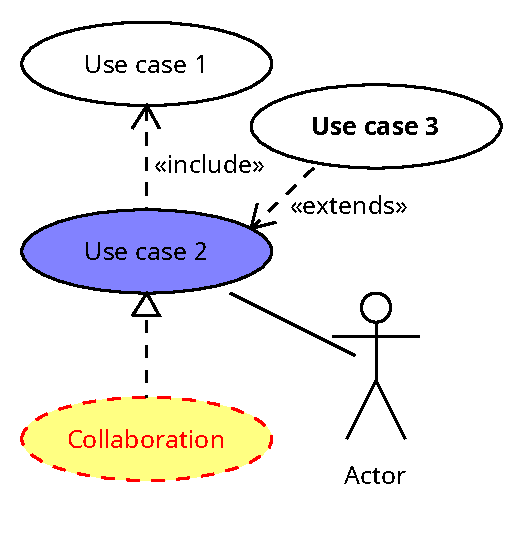
\includegraphics[width=\textwidth]{Diagrams/Diagram.pdf}
        \caption{Use case diagram}
        \label{fig:collaborative_filtering}
    \end{subfigure}
    \hfill
    \begin{subfigure}[b]{0.45\textwidth}
        \centering
        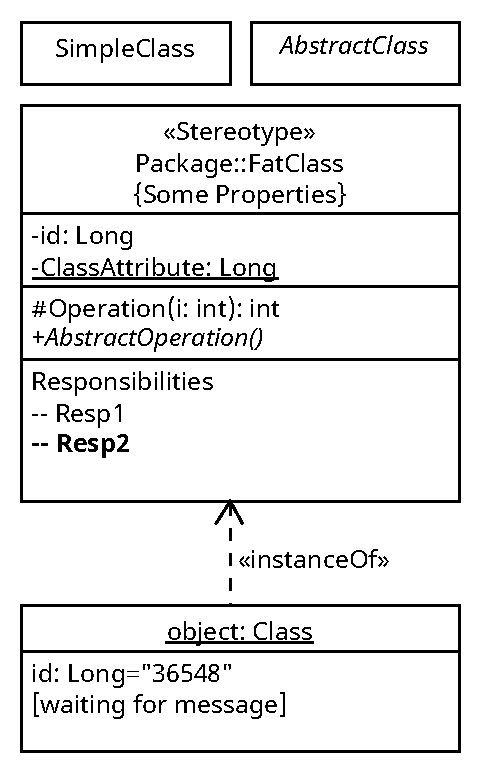
\includegraphics[width=\textwidth]{Diagrams/Diagram 2024-10-24 01-38-35.pdf}
        \caption{Class diagram}
        \label{fig:content_based_filtering}
    \end{subfigure}
    \caption{Comparison of Different Diagrams Used in Recommendation Systems}
    \label{fig:recommendation_systems}
\end{figure}

\begin{figure*}[htbp]
    \centering
    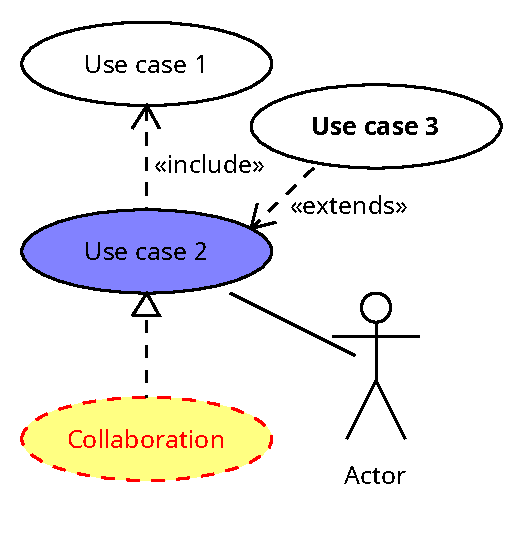
\includegraphics[width=\textwidth]{Diagrams/Diagram.pdf}
    \caption{Full Width Diagram}
    \label{fig:full_width_diagram}
\end{figure*}

\begin{equation}
    A = \begin{bmatrix}
        a_{11} & a_{12} & a_{13} & a_{14} \\
        a_{21} & a_{22} & a_{23} & a_{24} \\
        a_{31} & a_{32} & a_{33} & a_{34} \\
        a_{41} & a_{42} & a_{43} & a_{44} \\
        a_{51} & a_{52} & a_{53} & a_{54}
    \end{bmatrix}
\end{equation}

\begin{equation}
    S_n = \sum_{i=1}^{n} \frac{1}{i^2 + 1} + \frac{1}{i^3 + 1} + \frac{1}{i^4 + 1} + \ldots + \frac{1}{i^n + 1}
\end{equation}

\section{Záver} \label{zaver} % prípadne iný variant názvu



%\acknowledgement{Ak niekomu chcete poďakovať\ldots}


% týmto sa generuje zoznam literatúry z obsahu súboru literatura.bib podľa toho, na čo sa v článku odkazujete
\bibliographystyle{plain}
\bibliography{literatura}
\end{document}
